\documentclass[12 pt]{article}
\usepackage[margin = 1cm]{geometry}
\usepackage [utf8]{inputenc}
\usepackage[T2A]{fontenc}
\usepackage[russian]{babel}
\usepackage{amsthm, amsmath, amssymb}
\usepackage{xcolor}
\definecolor{mygreen}{rgb}{0,0.6,0}
\usepackage{listings}
\usepackage{graphicx}
\usepackage{hyperref}
\lstset{
  language=Java,
  tabsize=2,
  belowcaptionskip=1\baselineskip,
  breaklines=true,
  xleftmargin=1cm,
  escapechar=|,
  showstringspaces=false,
  commentstyle=\color{green},
  keywordstyle=\color{blue},
  stringstyle=\color{mygreen},
  basicstyle=\footnotesize\ttfamily,
  numbers=left,
  commentstyle=\usefont{T2A}{fcr}{m}{sl}
}

\renewcommand{\O}{\mathcal{O}}
\newcommand{\SO}{\Rightarrow}
\newcommand{\EQ}{\Leftrightarrow}
\newcommand{\union}{\cup}
\renewcommand{\div}{\mathop{\raisebox{-2pt}{\vdots}}}

\begin{document}
	Давайте напишем приложение, которое при смене местоположения отправлет запрос сайту с погодой, а потом выводит её пользователю. Начнём с той сущности, которая должна быть в любом приложении.
\section{Android Manifest}
    Манифест - файлик, лежащий в директории main.
    \begin{itemize}
    	\item В Manifest-файле описывается сам проект, в том числе настройки и конфигурации(например, версии проекта).
    	\item Права, которые должны запросить другие приложения для получения доступа к вашему приложению. 
    	\item Составляющие проекта, такие как:
		\begin{enumerate}
        	\item Activity 
        	\item BroadCastReceiver 
        	\item Service
        \end{enumerate}
        О них мы поговорим дальше.
    \end{itemize}
    
    Пока что наш манифест выглядит так:
    \begin{lstlisting}
<?xml version="1.0" encoding="utf-8"?>
<manifest xmlns:android="http://schemas.android.com/apk/res/android"
    package="edu.spbau.android.forecast" >

    <application
        android:allowBackup="true"
        android:icon="@mipmap/ic_launcher"
        android:label="@string/app_name"
        android:theme="@style/AppTheme" >
    </application>

</manifest>    
    \end{lstlisting}
    Внутри тега Application как раз должны быть описаны части приложения, а также устанавливаются настройки приложения. icon, label, theme - описывают значок приложения в меню телефона.
    
    В принципе, части приложения можно регистрировать и программно. Но мы этого касаться не будем.
\section{Activity}
    Поговорим о Activity. Activity - это окно приложения. Простые приложения состоят из одного Activity. Более сложные приложения могут иметь несколько окон, т.е. они состоят из нескольких Activity, которыми надо уметь управлять и которые могут взаимодействовать между собой.

    Activity, которая запускается первой, считается главной. Из Activity можно запустить другие Activity.

    Activity - это класс и у него есть некоторые методы, которые вызываются во время его жизни. Каждый Activity имеет определённый жизненный цикл:

<<<<<<< HEAD
	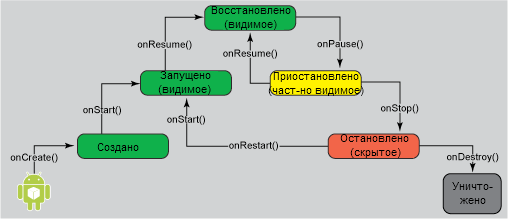
\includegraphics{LifeCycle.png}
=======
	\includegraphics{activity_lifecycle.png}
>>>>>>> 7257234cd4f8a1229a5d50f3966045f111454229
	
	Когда запускается Activity вызывается метод .onCreate(), потом .onStart() и потом .onResume(), затем приложение показывается на экране. Соответсвенно, ActivityRunning на картинке означает, что Activity на экране и с ним взаимодействует пользователь. Все статические действия(создание каких-нибудь классов, переменных) обычно делают в .onCreate(). Сбор окна приложения - создание элементов или загрузка Layout - обычно происходит в .onStart().
	
	.onPause - значит, что наше окно перекрылось каким-то другим, то есть оно есть, но не активно и пользователь с ним не взаимодействует. После того, как ему снова вернулась активность - снова взывается .onResume, таким образм, .onResume парное к onPause - если что-то надо выключить, когда приложение становится неактивным, то включать его надо в .onResume(). onStope() - парный к onStart() - надо освободить ресурсы. И onDestroy - к onCreate.
	
	Теперь, давайте посмотрим, как Activity прописывать в манифесте. У нас будут только одно окно - активити, а именно - главное. Таким образом, манифест сейчас выглядит так:
	
	\begin{lstlisting}
<?xml version="1.0" encoding="utf-8"?>
<manifest xmlns:android="http://schemas.android.com/apk/res/android"
    package="edu.spbau.android.forecast" >

    <application
        android:allowBackup="true"
        android:icon="@mipmap/ic_launcher"
        android:label="@string/app_name"
        android:theme="@style/AppTheme" >
        <activity
            android:name=".MainActivity"
            android:label="@string/app_name" >
            <intent-filter>
                <action android:name="android.intent.action.MAIN" />

                <category android:name="android.intent.category.LAUNCHER" />
            </intent-filter>
        </activity>    
    </application>
</manifest>
    \end{lstlisting}
    
    Прописывая Activity, мы также прописывает intent, на который он реагирует. Intent - класс, позволяющий частям приложения общаться между собой(или между приложениями). В нашем случае, когда пользователь нажимает на иконку приложения в меню, приложению посылается Intent MAIN. Поэтому, мы говорим, что наше Activity реагирует на intent Main, а категория intent-а говорит о том, что Activity надо запустить.
    
    Разберём по частям наше Activity. 
    
    \begin{lstlisting}
public class MainActivity extends ActionBarActivity {

    private LocationManager mLocationManager;
    private PendingIntent mLocationChangedIntent;

    @Override
    protected void onCreate(Bundle savedInstanceState) {
        ...
    }

    @Override
    protected void onResume() {
        ...
    }

    @Override
    protected void onPause() {
        ...
    }


    @Override
    public boolean onCreateOptionsMenu(Menu menu) {
        ...
    }

    @Override
    public boolean onOptionsItemSelected(MenuItem item) {
        ...
    }

}
    \end{lstlisting}
    
    mLocationManager - поле, которое будет хранить в себе специальный класс, с помощью которого мы будем узнавать о нашем местоположении. 
    
    mLocationChangedIntent - это поле класса PendingIntent, котороый делает почти то же, что и Intent, с помощью него мы потом запустим другую часть нашего приложения. Единственное отличие PendingIntent от Intent - это то, что когда PendingIntent запускает какую-нибудь сущность, то она запускается с правами исходного приложения. 
<<<<<<< HEAD
    
    Мы наследуемся от ActionBarActivity - которая добавляет полосочку(ActionBar) наверху экрана. Там есть меню, которое раскрывается, а onOptionsItemSelected обрабатывает нажатие на какой-то пункт. onCreateOptionsMenu - вызывается при создании ActionBar. Причём, если он вернёт false, то меню не покажется, а если true - то отрисуется. onOptionsItemSelected должно возвращать true, если у него получилось обработать событие.
    
    Реализуем их:
    
    \begin{lstlisting}
@Override
public boolean onCreateOptionsMenu(Menu menu) {
    getMenuInflater().inflate(R.menu.menu_main, menu);
    return true;
}

@Override
public boolean onOptionsItemSelected(MenuItem item) {
    int id = item.getItemId();

    if (id == R.id.action_settings) {
        return true;
    }

    return super.onOptionsItemSelected(item);
}    
    \end{lstlisting} 
    
    Здесь мы в функции onCreateOptionsMenu говорим, что Menu будет рисоваться так, как мы это описали в layout(это xml файлики, описывающие разметку), а в onOptionsItemSelected - в if обрабатывается действие нажатия на конкретный пункт меню. В данном случае, мы ничего не делаем, просто говорим true - обработали. Можно передать обработку нажатия на пункт меню нашему предку, что мы и делаем во всех остальных случаях.
    
    Все layouts для Activity лежат в директории main/res/layout. А layout для menu лежит в main/res/menu. Наш файлик-xml назыается menu\_main.xml(собственно, по этому имени и происходит загрузка этого layout как разметки для меню). В файлике:
    
    \begin{lstlisting}
<menu
    xmlns:android="http://schemas.android.com/apk/res/android"
    xmlns:app="http://schemas.android.com/apk/res-auto"
    xmlns:tools="http://schemas.android.com/tools"
    tools:context=".MainActivity">

    <item
        android:id="@+id/action_settings"
        android:title="@string/action_settings"
        android:orderInCategory="100"
        app:showAsAction="never" />

</menu>    
    \end{lstlisting}
    
    У нас ровно 1 пункт в меню, описывающийся в теге item. Мы настроили для него title(строка, которая отображаетсяв меню), его id - по нему мы находим этот item в onOptionsItemSelected, и другие.
    
    В андроиде принято все константы хранить в директории res/values. И использовать переменные, им соответсвующие. Там же(в res/values) есть специальное место для хранения строковых литералов, называется файл strings.xml. Там мы храним строковые литералы. Вот наш файлик:
    
    \begin{lstlisting}
<resources>
    <string name="app_name">Forecast</string>
    <string name="action_settings">Settings</string>
</resources>   
    \end{lstlisting}
    
    Как видно, мы храним строковый литерал "Settings" в переменной action\_settings. И для описания item в нашем layout для меню мы используем переменную, хранящую этот литерал.
    
    Идём дальше. Рассмотрим метод onCreate() нашей Activity:
    
    \begin{lstlisting}
@Override
protected void onCreate(Bundle savedInstanceState) {
    super.onCreate(savedInstanceState);
    setContentView(R.layout.activity_main);
    if (savedInstanceState == null) {
        getSupportFragmentManager().beginTransaction()
                .add(R.id.container, new ForecastFragment())
                .commit();
    }

    mLocationManager = (LocationManager) getSystemService(Context.LOCATION_SERVICE);
    Intent intent = new Intent(this, LocationChangedReceiver.class);
    mLocationChangedIntent =
            PendingIntent.getBroadcast(this, 0, intent, PendingIntent.FLAG_UPDATE_CURRENT);
}   
    \end{lstlisting}  
    
    Класс Bundle создаётся для сохранения важной информации(например, пользовательского UI), в onCreate его можно восстановить. А onSaveInstanceState(Bundle savedInstanceState) можно переопределить и добавит в Bundle ещё что-то своё. Вызывается onSaveInstanceState перед onPause(). Но нам сейчас это не особенно важно - важно, что обязательно надо вызвать тот же метод у супер-класса.
    
=======
    
    Мы наследуемся от ActionBarActivity - которая добавляет полосочку(ActionBar) наверху экрана. Там есть меню, которое раскрывается, а onOptionsItemSelected обрабатывает нажатие на какой-то пункт. onCreateOptionsMenu - вызывается при создании ActionBar. Причём, если он вернёт false, то меню не покажется, а если true - то отрисуется. onOptionsItemSelected должно возвращать true, если у него получилось обработать событие.
    
    Реализуем их:
    
    \begin{lstlisting}
@Override
public boolean onCreateOptionsMenu(Menu menu) {
    getMenuInflater().inflate(R.menu.menu_main, menu);
    return true;
}

@Override
public boolean onOptionsItemSelected(MenuItem item) {
    int id = item.getItemId();

    if (id == R.id.action_settings) {
        return true;
    }

    return super.onOptionsItemSelected(item);
}    
    \end{lstlisting} 
    
    Здесь мы в функции onCreateOptionsMenu говорим, что Menu будет рисоваться так, как мы это описали в layout(это xml файлики, описывающие разметку), а в onOptionsItemSelected - в if обрабатывается действие нажатия на конкретный пункт меню. В данном случае, мы ничего не делаем, просто говорим true - обработали. Можно передать обработку нажатия на пункт меню нашему предку, что мы и делаем во всех остальных случаях.
    
    Все layouts для Activity лежат в директории main/res/layout. А layout для menu лежит в main/res/menu. Наш файлик-xml назыается menu\_main.xml(собственно, по этому имени и происходит загрузка этого layout как разметки для меню). В файлике:
    
    \begin{lstlisting}
<menu
    xmlns:android="http://schemas.android.com/apk/res/android"
    xmlns:app="http://schemas.android.com/apk/res-auto"
    xmlns:tools="http://schemas.android.com/tools"
    tools:context=".MainActivity">

    <item
        android:id="@+id/action_settings"
        android:title="@string/action_settings"
        android:orderInCategory="100"
        app:showAsAction="never" />

</menu>    
    \end{lstlisting}
    
    У нас ровно 1 пункт в меню, описывающийся в теге item. Мы настроили для него title(строка, которая отображаетсяв меню), его id - по нему мы находим этот item в onOptionsItemSelected, и другие.
    
    В андроиде принято все константы хранить в директории res/values. И использовать переменные, им соответсвующие. Там же(в res/values) есть специальное место для хранения строковых литералов, называется файл strings.xml. Там мы храним строковые литералы. Вот наш файлик:
    
    \begin{lstlisting}
<resources>
    <string name="app_name">Forecast</string>
    <string name="action_settings">Settings</string>
</resources>   
    \end{lstlisting}
    
    Как видно, мы храним строковый литерал "Settings" в переменной action\_settings. И для описания item в нашем layout для меню мы используем переменную, хранящую этот литерал.
    
    Идём дальше. Рассмотрим метод onCreate() нашей Activity:
    
    \begin{lstlisting}
@Override
protected void onCreate(Bundle savedInstanceState) {
    super.onCreate(savedInstanceState);
    setContentView(R.layout.activity_main);
    if (savedInstanceState == null) {
        getSupportFragmentManager().beginTransaction()
                .add(R.id.container, new ForecastFragment())
                .commit();
    }

    mLocationManager = (LocationManager) getSystemService(Context.LOCATION_SERVICE);
    Intent intent = new Intent(this, LocationChangedReceiver.class);
    mLocationChangedIntent =
            PendingIntent.getBroadcast(this, 0, intent, PendingIntent.FLAG_UPDATE_CURRENT);
}   
    \end{lstlisting}  
    
    Класс Bundle создаётся для сохранения важной информации(например, пользовательского UI), в onCreate его можно восстановить. А onSaveInstanceState(Bundle savedInstanceState) можно переопределить и добавит в Bundle ещё что-то своё. Вызывается onSaveInstanceState перед onPause(). Но нам сейчас это не особенно важно - важно, что обязательно надо вызвать тот же метод у супер-класса.
    
>>>>>>> 7257234cd4f8a1229a5d50f3966045f111454229
     setContentView - устанавливает разметку Activity, мы загружаем её из xml файла в директории layout, как говорилось ранее - в layout хранятся разметки для Activity.
     
     В mLocationManager мы получаем LocationManager.
     
     Далее создаём Intent, на который будет реагировать только класс LocationChangedReceiver, а затем посылаем его. PandingIntent.getBroadcast преобразует Intent в PendingIntent, а затем посылает его всем. Но мы задали, что реагировать на него будет только LocationChangedReceiver, поэтому он придёт только туда. Мы используем метод .getBroadcast, так как получатель - класс BroadCastReceiver(мы рассмотрим его дальше). Есть также методы .getActivity, .getService. 
     
     Впоследствии мы будет использовать этот PendingIntent. FLAG\_UPDATE\_CURRENT нужен для того, чтобы мы могли извещать PendingIntent об изменениях в нашем местоположении. Когда будем записывать наше местоположение в PendingIntent, он будет заново рассылаться. Проще говоря, флаг говорит о том, что когда кто-нибудь измененяет данные PendingIntent, он отправляется всем очередной раз.
     
     Теперь рассмотрим:
     
     \begin{lstlisting}
@Override
protected void onResume() {
    super.onResume();

    final int FIVE_MINUTES = 5 * 60 * 1000;

    mLocationManager.requestLocationUpdates(LocationManager.GPS_PROVIDER,
            FIVE_MINUTES, 0, mLocationChangedIntent);
}    
     \end{lstlisting}
    
    Заметим, что во всех методах жизненного цикла необходимо вызвать тот же у предка. Так было с onCreate, onResume, так будет и с остальными. Наш метод onResume довольно прост - он просит LocationManager дёргать наш PendingIntent раз в 5 минут и класть туда информацию о местоположении, первый параметр говорит какое устройство нам передаёт информацию, а третий - минимальная разница в метрах, при которых мы считаем произошёл update. В данном случае - мы будем дёргать Intent всегда.
    
    OnPause метод у нас будет тоже довольно простой:
    \begin{lstlisting}
@Override
protected void onPause() {
    super.onPause();
    mLocationManager.removeUpdates(mLocationChangedIntent);
} 
    \end{lstlisting}
    
    Мы просто вызываем тот же метод у предка(как и для любого метода из жизненного цикла), а потом останавливаем оповещение PendingIntent об изменении в текущем положении - при методе onPause, Activity не активно, часто не видно, поэтому нам не надо обновлять информацию.
    
    Вот и всё. Мы не будет переопределять onStope и onDestroy, так как в данном случае это не требуется.
\section{BroadCastReceiver} 
    Ещё помните, куда мы там посылали наш PendingIntent? В класс BroadCastReceiver! Вот как раз о нём мы сейчас и поговорим.
    
    BroadCastReceiver - класс-обработчик широковещательных сообщений(intent). Может быть подписан на несколько разных интентов. Когда приходит интент, BroadCastReceiver-ы, подписанные на него, выстраиваются в цепочку в соответствии с приоритетами. И если один из BroadcastReceiver-ов обрабатывает сообщение слишком долго, то другие вынуждены ждать. Поэтому Android прерывает исполнение BroadCastReceiver-ов, которые работают больше определённого времени. Из-за этого количество действий, которое вы можете сделать с помощью BroadCastReceiver, довольно ограничено(обычное использование - послать другой интент, чтобы запустить Activity, Service или что-нибудь подобное).
    
    Другое назначение BroadCastReceiver это получать системные оповещения, такие как оповещения о маленьком заряде батарейки или о том, что Android загрузился.
    
    BroadCastReceiver региструется в Android Manifest'е так:
    \begin{lstlisting}
<receiver android:name=".LocationChangedReceiver" />
    \end{lstlisting} 
    
    Таким образом, наш Manifest-файл теперь будет такой:
    
    \begin{lstlisting}
<?xml version="1.0" encoding="utf-8"?>
<manifest xmlns:android="http://schemas.android.com/apk/res/android"
    package="edu.spbau.android.forecast" >

    <application
        android:allowBackup="true"
        android:icon="@mipmap/ic_launcher"
        android:label="@string/app_name"
        android:theme="@style/AppTheme" >
        <activity
            android:name=".MainActivity"
            android:label="@string/app_name" >
            <intent-filter>
                <action android:name="android.intent.action.MAIN" />

                <category android:name="android.intent.category.LAUNCHER" />
            </intent-filter>
        </activity>

        <receiver android:name=".LocationChangedReceiver" />
    </application>

</manifest>   
    \end{lstlisting}
    
    Как понятно из Manifest-файла, имя нашего BroadCastReceiver будет LocationChangedReceiver.
        
    Указать, на какие intent'ы подписан BroadCastReceiver, можно двумя способами:
	\begin{itemize}
    	\item В Android Manifest (обычно при подписке на системные события)
		\item Программно:
        \begin{lstlisting}
mLocationManager = (LocationManager)getSystemService(Context.LOCATION_SERVICE);
Intent intent = new Intent(this, LocationChangedReceiver.class);
mLocationChangedIntent =
PendingIntent.getBroadcast(this, 0, intent, PendingIntent.FLAG_UPDATE_CURRENT);
    \end{lstlisting} - как мы и делали.
    \end{itemize}

    Посмотрим на наш BroadCastReceiver:
            \begin{lstlisting}
public class LocationChangedReceiver extends BroadcastReceiver {

    private static final String TAG = LocationChangedReceiver.class.getSimpleName();

    public LocationChangedReceiver() { }

    @Override
    public void onReceive(Context context, Intent intent) {
        final String locationKey = LocationManager.KEY\_LOCATION\_CHANGED;

        if (intent.hasExtra(locationKey)) {
            Location location = (Location) intent.getExtras().get(locationKey);

            Intent startService = new Intent(context, ForecastUpdateService.class);
            startService.putExtra(LocationManager.KEY_LOCATION_CHANGED, location);
            context.startService(startService);
        }
    }
}
    \end{lstlisting}

      Теперь пришло время поговорить об Intent-ах чуть подробнее. Все Intent могут хранить в себе информацию. Добавлять её можно вручную - у Intent есть специальные методы .putExtra(String key, ...) - где второй параметр это то, что мы хотим добавить. Эти методы определены для основных классов Java. Полный список методов можно найти тут: \href{https://developer.android.com/reference/android/content/Intent.html}{тык}
    
        И, если кто-то реагирует на Intent с данными и начинает его обрабатывать, то мы можем из Inent вытащить дополнительную информацию. 
        
        Когда приходит интент, который предназначен для данного BroadCastReceiver, вызывается метод onReceive(). 
        
        Одним из его аргументов является экземпляр класса Context - базовый класс для частей приложения. Через него можно обращаться к ресурсам Android. К примеру, Activity - наследник класса Context. Поэтому, мы можем вызвать, например, метод getSystemService(), определённый в классе Context - для доступа к какому-то сервису. А вот BroadCastReceiver не является наследником класса Context, но доступ к различным менеджерам может понадобиться, поэтому контекст и передаётся методу onReceive(). Наследниками Context также являются разнообразные Service и Activity классы(например, IntentService или AliasActivity).
        
        Вторым аргументом является Intent, на который он среагировал. Мы берём этот интент и вытаскиваем из него информацию, которую положил туда LocationManager. Известно, что LocationManager при вызванном нами методе кладёт информацию с ключом LocationManager.KEY\_LOCATION\_CHANGED(это можно найти в документации), поэтому мы и достаём оттуда значение по этому ключу. .getExtras возвращает Bundle - специальный класс для хранение данных вида ключ(строка)-значение(Object). Так что .get() возвращает Object, его надо прикастовать к Location - класс, в котором содержитьс информация о нашем местоположении.
     
    Дальше, в силу скромных возможностей BroadCastReceiver мы перенаправляем запрос классу Service. Про этот класс мы поговорим дальше.
    
    Чтобы передать управление классу Service, мы также используем Intent. Здесь мы используем обычный Intent, и всё работает. Но почему мы не могли создать обычный интент при обработке LocationManager-ом? Всё дело в том, что LocationManager принимает только PendingIntent, поэтому нам пришлось идти длинным путём.
    
    Итак, мы создали интент ручками и указали класс, который на него подписан - ForecastUpdateService. Дальше положили полученную информацию уже в новый интент и отправили сервису. Это можно сделать с помощью команды startService. А если бы мы отправляли интент Activity, то метод назывался бы startActivity - осторожно!
            
\section{Log}     
    Наверняка вы заметили странное статическое поле в BroadCastReceiver: 
    \begin{lstlisting}
private static final String TAG = LocationChangedReceiver.class.getSimpleName();
    \end{lstlisting}
    
    Оно используется для логирования.
    
    \begin{itemize}
        \item Записи в log выводятся на экран Device Monitor.Logcat.
        \item Логирование происходит так:
    \end{itemize}
    \begin{lstlisting}
    ...
private static final String TAG = 
            SMSReceiver.class.getSimpleName();
    ...
Log.d(TAG, "SMS received");    
    \end{lstlisting}

    В нашем случае мы ничего не логируем, но в целом логирование - хороший тон.
    
    \section{Service}    
    Теперь, наконец, поговорим про Service.
    
    \begin{itemize}
        \item Service также надо прописывать в манифесете:
        \begin{lstlisting}
<service
    android:name=".DatabaseService"
    android:exported="false" >
</service>        
        \end{lstlisting}
        
        Таким образом, в нашем манифест-файле теперь появилась новая сущность:
        \begin{lstlisting}
<?xml version="1.0" encoding="utf-8"?>
<manifest xmlns:android="http://schemas.android.com/apk/res/android"
    package="edu.spbau.android.forecast" >

    <application
        android:allowBackup="true"
        android:icon="@mipmap/ic_launcher"
        android:label="@string/app_name"
        android:theme="@style/AppTheme" >
        <activity
            android:name=".MainActivity"
            android:label="@string/app_name" >
            <intent-filter>
                <action android:name="android.intent.action.MAIN" />

                <category android:name="android.intent.category.LAUNCHER" />
            </intent-filter>
        </activity>

        <receiver android:name=".LocationChangedReceiver" />

        <service
            android:name=".ForecastUpdateService"
            android:exported="false" />
    </application>

</manifest>        
        \end{lstlisting}
        Ключ exported задаёт, позволено ли другим приложениям запускать наш сервис, Activity и тд. В нашем случае - не позволено.
        \item Если intent занят какой-то другой сущностью, то Service также становится в очередь.
        \item При обработке intent запускается метод onHandleIntent(Intent intent);
    \end{itemize}
    
    Давайте разберём, что мы здесь делаем:
    \begin{lstlisting}
public class ForecastUpdateService extends IntentService {

    private final static String TAG = ForecastUpdateService.class.getSimpleName();

    public ForecastUpdateService() {
        super(TAG);
    }

    private void parseJsonData(String json) {
        final String JSON_LIST = "list";
        final String JSON_SPEED = "speed";
        final String JSON_DEGREE = "deg";
        final String JSON_TEMPERATURE = "temp";
        final String JSON_DAY_TEMPERATURE = "day";
        final String JSON_NIGHT_TEMPERATURE = "night";
        final String JSON_WEATHER = "weather";
        final String JSON_WEATHER_ID = "id";

        try {
            JSONObject forecastJson = new JSONObject(json);
            JSONArray weatherArray = forecastJson.getJSONArray(JSON_LIST);

            ArrayList<ContentValues> forecast = new ArrayList<>(weatherArray.length());

            Time dayTime = new Time();
            dayTime.setToNow();
            int julianStartDay = Time.getJulianDay(System.currentTimeMillis(), dayTime.gmtoff);
            dayTime = new Time();

            for(int i = 0; i < weatherArray.length(); i++) {
                JSONObject dayForecast = weatherArray.getJSONObject(i);

                long dateTime = dayTime.setJulianDay(julianStartDay + i);

                double speed = dayForecast.getDouble(JSON_SPEED);
                double degree = dayForecast.getDouble(JSON_DEGREE);

                JSONObject temperatureObject = dayForecast.getJSONObject(JSON_TEMPERATURE);
                double day = temperatureObject.getDouble(JSON_DAY_TEMPERATURE);
                double night = temperatureObject.getDouble(JSON_NIGHT_TEMPERATURE);

                JSONArray weatherObjects = dayForecast.getJSONArray(JSON_WEATHER);
                JSONObject weatherObject = weatherObjects.getJSONObject(0);
                int weather = weatherObject.getInt(JSON_WEATHER_ID);

                ContentValues weatherValues = new ContentValues();
                weatherValues.put(WeatherContract.WeatherEntry.COLUMN_DATE, dateTime);
                weatherValues.put(WeatherContract.WeatherEntry.COLUMN_DEGREES, degree);
                weatherValues.put(WeatherContract.WeatherEntry.COLUMN_WIND_SPEED, speed);
                weatherValues.put(WeatherContract.WeatherEntry.COLUMN_NIGHT_TEMP, night);
                weatherValues.put(WeatherContract.WeatherEntry.COLUMN_DAY_TEMP, day);
                weatherValues.put(WeatherContract.WeatherEntry.COLUMMN_WEATHER_ID, weather);
                forecast.add(weatherValues);
            }

            if (forecast.size() > 0) {
                ContentValues values[] = new ContentValues[forecast.size()];
                forecast.toArray(values);
                getContentResolver().bulkInsert(WeatherContract.WeatherEntry.CONTENT_URI, values);
            }
        } catch (JSONException e) {
            Log.e(TAG, "Error while parsing JSON", e);
        }
    }

    @Override
    protected void onHandleIntent(Intent intent) {
        final String locationKey = LocationManager.KEY_LOCATION_CHANGED;

        final String FORECAST_BASE_URL =
                "http://api.openweathermap.org/data/2.5/forecast/daily?";
        final String LATITUDE_PARAM = "lat";
        final String LONGITUDE_PARAM = "lon";
        final String MODE_PARAM = "mode";
        final String JSON = "json";
        final String UNITS_PARAM = "units";
        final String METRIC = "metric";

        if (!intent.hasExtra(locationKey)) {
            Log.w(TAG, "Received intent without location");
            return;
        }

        Location location = (Location) intent.getExtras().get(locationKey);
        HttpURLConnection connection = null;
        BufferedReader reader = null;

        try {
            Uri uri = Uri.parse(FORECAST_BASE_URL).buildUpon()
                    .appendQueryParameter(LATITUDE_PARAM, Double.toString(location.getLatitude()))
                    .appendQueryParameter(LONGITUDE_PARAM, Double.toString(location.getLongitude()))
                    .appendQueryParameter(MODE_PARAM, JSON)
                    .appendQueryParameter(UNITS_PARAM, METRIC).build();
            URL url = new URL(uri.toString());
            connection = (HttpURLConnection) url.openConnection();
            connection.setRequestMethod("GET");
            connection.connect();

            InputStream inputStream = connection.getInputStream();
            StringBuilder buffer = new StringBuilder();
            if (inputStream == null) {
                return;
            }
            reader = new BufferedReader(new InputStreamReader(inputStream));
            String line;
            while ((line = reader.readLine()) != null) {
                buffer.append(line);
                buffer.append("\n");
            }

            if (buffer.length() == 0) {
                return;
            }

            parseJsonData(buffer.toString());
        } catch (IOException e) {
            Log.e(TAG, "Error", e);
        } finally {
            if (reader != null) {
                try {
                    reader.close();
                } catch (IOException e) {
                    Log.e(TAG, "Error while closing stream", e);
                }
            }
            if (connection != null) {
                connection.disconnect();
            }
        }
    }

}
    \end{lstlisting}
    
    Выглядит страшно, но скоро всё будет понятно. Начнём сначала, вот Intent начинает обрабатывать функция onHandleIntent. Первым делом мы задаём некоторые значения, которые впоследствии могут нам понадобиться - первое для извлечение локации из Intent. Остальные - специальные параметры для декодирования и кодирования определённых форматов.
    
    Дальше мы проверяем, что пришёдший интент действительно содержит нужную информацию(функция hasExtra(String key)), и если нет - используем логирование, чтобы сообщить об ошибке и выходим. Мы уже умные, мы знаем, что это такое. 
    
    Если информация в Intent действительно содержиться, мы извлекаем информацию в location. Дальше нам нужно подключиться по интернету. Но для этого нужны некоторые права.
    
\section{Permissions}
    \begin{itemize}
        \item Чтобы работать с сетью надо подключить соотетсвующие permission.
        \begin{lstlisting}
<uses-permission android:name="android.permission.INTERNET" /> 
<uses-permission  android:name="android.permission.ACCESS_NETWORK_STATE"/>        
        \end{lstlisting}
        
        Таким образом, манифест-файл выглядит сейчас так:
        \begin{lstlisting}
<?xml version="1.0" encoding="utf-8"?>
<manifest xmlns:android="http://schemas.android.com/apk/res/android"
    package="edu.spbau.android.forecast" >

    <uses-permission android:name="android.permission.ACCESS_FINE_LOCATION" />
    <uses-permission android:name="android.permission.INTERNET" />
    <uses-permission android:name="android.permission.ACCESS_NETWORK_STATE" />

    <application
        android:allowBackup="true"
        android:icon="@mipmap/ic_launcher"
        android:label="@string/app_name"
        android:theme="@style/AppTheme" >
        <activity
            android:name=".MainActivity"
            android:label="@string/app_name" >
            <intent-filter>
                <action android:name="android.intent.action.MAIN" />

                <category android:name="android.intent.category.LAUNCHER" />
            </intent-filter>
        </activity>

        <receiver android:name=".LocationChangedReceiver" />

        <service
            android:name=".ForecastUpdateService"
            android:exported="false" />
    </application>
</manifest>        
        \end{lstlisting}
        \item Для получени данных относительно точной локации, также нужно разрешение - оно первое в списке.
        \item Второе позволяет открывать сетевые сокеты.
        \item А третье позволяет приложениям получать доступ к информации о сетях.
    \end{itemize}
    
\section{Connection}

    Продолжим разбираться с нашим Service. Мы остановились на том, что мы хотим выйти в сеть.
    \begin{itemize}
        \item Самый простой способ работать с сетью - это HttpURLConnection. Сначала мы долго-долго строим URL-адрес, в котором находится наш запрос - мы достаём из Location широту и долготу, а потом получаем HttpURLConnection по этому URL. Возвращается методом .openConnection():
        \begin{lstlisting}
URL url = new URL(uri.toString());
connection = 
        (HttpURLConnection) url.openConnection();
        \end{lstlisting}
        Здесь нужен каст, так как .openConnection на самом деле возвращает URLConnection, но по факту это - HttpURLConnection, так как наш сайт работает по протоколу http.
        \item Протокол http может обрабатывать различные запросы. Например, запрос на получение информации. Если мы хотим получить информацию - пишем следующее:
        \begin{lstlisting}
connection.setRequestMethod("GET");
        \end{lstlisting}
        А мы действительно хотим получить информацию по запросу, который мы отправили вместе c URL.
        Затем мы собственно, создаём соединение - функцией connection.connect();
    \end{itemize}
    Несложно, да? Мы создали соединение на основе connection. Осталось оттуда прочитать данные.
    Считываем информацию мы так:
    \begin{lstlisting}
InputStream inputStream = connection.getInputStream();
StringBuilder buffer = new StringBuilder();
if (inputStream == null) {
    return;
}
reader = new BufferedReader(new InputStreamReader(inputStream));
String line;
while ((line = reader.readLine()) != null) {
    buffer.append(line);
    buffer.append("\n");
}

if (buffer.length() == 0) {
    return;
}
    \end{lstlisting}
    
    А теперь пояснение. Мы берём InputStream, связанный с нашим соединением. Прочитаем всё в StringBuilder - мы будем читать строчками, поэтому нам надо сконкатенировать. StringBuilder здесь лучший выбор. Чтобы удобнее было работать с потоком чтения, мы оборачиваем его в BufferedReader - и читаем построчно, пока не закончаться строчки. Если ничего не пришло, то длина buffer окажется равной нулю - и мы выходим.
    
    Отлично, теперь у нас есть StringBuilder из строчек результата. Ответ надо распарсить.
    
    Обычно ответ формируется либо в формате xml, либо в формате json - это два разных представления данных. В данном случае, мы используем json. Нужно этот формат распарсить и обработать - для этого мы написали функцию parseJsonData(String), но подробно на ней останавливаться не будем. Для этого пришлось бы углубиться ещё и в структуру формата json и API сайта. После этого, в onHandleIntent мы обрабатываем все ошибки, а в блоке finally закрывает открытые ресурсы.
    
    Что важно не пропустить в parseJsonData - последний if - если данные о погоде есть, то мы их куда-то вставляем. В будущем мы поймём, что куда-то - это базы данных.

\section{Data bases}
    
    Каждый раз при смене своих координат не очень разумно слать запрос в интернет. Это долго, это не надёжно - интернет или сервис могут не работать. Поэтому стоит задуматься о том, как приложение будет работать в offline-режиме. К примеру, разумный вариант - когда у нас есть доступ к сети, получать погоду и сохранять её в базу данных. А когда сети нет - просто достаём из базы данных самое актуальное значение и показываем. Оно, может быть, и устаревшее, но хоть какое-то. Соответсвенно, следующая наша цель - получить результат и сохранить его в базу данных.
    
    В нашем проекте есть такой класс WeatherProvider - наследник класса ContentProvider.
	\begin{itemize}
		\item ContentProvider - это такой класс-обёртка над базой данных.
		\item Его также надо прописывать в манифесте:
		\begin{lstlisting}
<provider
	android:authorities="edu.spbau.android.forecast"
    android:name=".WeatherProvider" />		
		\end{lstlisting}
		android:authorities - обязательно должен быть и должен указывать путь к провайдеру(проще - пакет провайдера).
		
		Таким образом, манифест получается такой:
		\begin{lstlisting}
<?xml version="1.0" encoding="utf-8"?>
<manifest xmlns:android="http://schemas.android.com/apk/res/android"
    package="edu.spbau.android.forecast" >

    <uses-permission android:name="android.permission.ACCESS_FINE_LOCATION" />
    <uses-permission android:name="android.permission.INTERNET" />
    <uses-permission android:name="android.permission.ACCESS_NETWORK_STATE" />

    <application
        android:allowBackup="true"
        android:icon="@mipmap/ic_launcher"
        android:label="@string/app_name"
        android:theme="@style/AppTheme" >
        <activity
            android:name=".MainActivity"
            android:label="@string/app_name" >
            <intent-filter>
                <action android:name="android.intent.action.MAIN" />

                <category android:name="android.intent.category.LAUNCHER" />
            </intent-filter>
        </activity>

        <receiver android:name=".LocationChangedReceiver" />

        <service
            android:name=".ForecastUpdateService"
            android:exported="false" />
        
        <provider
            android:authorities="edu.spbau.android.forecast"
            android:name=".WeatherProvider" />
    </application>

</manifest>		
		\end{lstlisting}
		
		Это - окончательный вариант и больше он меняться не будет.
	\end{itemize}    
	
\section{Contract}
	
	Перд тем, как подробней говорить о ContentProvider, познакомимся с ещё одним классом Contract, реализация которого является правилом хорошего тона. Там обычно описывается структура базы данных. То есть, он необязателен, чтобы работать с базами данных, но лучше его реализовывать.
	
	Соответсвенно:
	\begin{itemize}
	    \item Его не надо прописывать в манифесте, так как это вспомогательный класс.
	    \item Там как константы хранятся названия таблиц, названия колонок, строк и другая подобная информация.
	    \item Для каждой таблички внутри контракта заводится класс-наследник интерфейса BaseColumns. И в нём уже описывается вся информация о конкретной табличке. 
	    \item В нашей базе данных будет только одна табличка, в которой будет храниться прогноз погоды по времени.
	\end{itemize}
	
	Наш Contract выглядит так:
	\begin{lstlisting}
public class WeatherContract {

    public static final String CONTENT_AUTHORITY = "edu.spbau.android.forecast";
    public static final Uri BASE_CONTENT_URI = Uri.parse("content://" + CONTENT_AUTHORITY);
    public static final String PATH_WEATHER = "weather";

    public static long normalizeDate(long gmt) {
        Time time = new Time();
        time.set(gmt);
        int day = Time.getJulianDay(gmt, time.gmtoff);
        return time.setJulianDay(day);
    }

    public static final class WeatherEntry implements BaseColumns {

        public static final Uri CONTENT_URI =
                BASE_CONTENT_URI.buildUpon().appendPath(PATH_WEATHER).build();

        public static final String CONTENT_TYPE =
                ContentResolver.CURSOR_DIR_BASE_TYPE + "/" + CONTENT_AUTHORITY + "/" + PATH_WEATHER;

        public static final String CONTENT_ITEM_TYPE =
                ContentResolver.CURSOR_ITEM_BASE_TYPE + "/" + CONTENT_AUTHORITY + "/" + PATH_WEATHER;

        public static final String TABLE_NAME = "weather";

        public static final String COLUMN_DATE = "date";
        public static final String COLUMN_DAY_TEMP = "day_temp";
        public static final String COLUMN_NIGHT_TEMP = "nigh_temp";
        public static final String COLUMN_WIND_SPEED = "wind";
        public static final String COLUMN_DEGREES = "direction";
        public static final String COLUMMN_WEATHER_ID = "weather_id";

        public static long getDateFromUri(Uri uri) {
            return Long.parseLong(uri.getPathSegments().get(1));
        }

        public static Uri buildWeatherUri(long date) {
            return ContentUris.withAppendedId(CONTENT_URI, date);
        }

    }

}	
	\end{lstlisting}
	
	В классе WeatherContract:
	\begin{itemize}
	    \item CONTENT\_AUTHORITY - путь к ContentProvider, иначе - пакет ContentProvider(в нашем случае - WeatherProvider)
	    \item BASE\_CONTENT\_URI - URI по пути к ContentProvider
	    \item PATH\_WEATHER - локальный путь к табличке weather. Чаще всего, просто название табличик. А так из локального пути к табличке и URI ContentProvider можно построить полный путь до таблички: 
	    \begin{lstlisting}
	    public static final Uri CONTENT_URI =
                BASE_CONTENT_URI.buildUpon().appendPath(PATH_WEATHER).build();
        \end{lstlisting}
	    \item public static long normalizeDate(long gmt) - как понятно из названия, нормализует время.
	    \item Подкласс, соотетсвующий нашей единственной табличке.
	    В нём:
	    \begin{itemize}
	        \item public static final Uri CONTENT\_URI -- Uri, по которому мы будем обращаться к конкретной табличке ContentProvider, так как доступ к ContentProvider осуществляется только через Uri. В данном случае - табличка, называющаяся weather.
	        \item public static final String CONTENT\_TYPE -- тип набора записей в ContentProvider.
	        \item public static final String CONTENT\_ITEM\_TYPE -- тип одной записи в ContentProvider
	        \item А затем разные атрибуты, описывающие табличку - её название, и колонки, которые в ней есть.
	        \item Также, в классе прописываются разные служебные методы. У нас реализованы преобразование даты в Uri, и наоборот. Чтобы мы смогли потом обратиться к какой-то записи, соотетсвующей определённой дате.
	    \end{itemize}
	    Выражения для CONTENT\_TYPE и CONTENT\_ITEM\_TYPE вегда одни и те же, но их всё равно приходится прописывать.
	\end{itemize}

\section{SQLiteOpenHelper}	

	Следующий класс, про который мы поговорим перед ContentProvider, это абстрактный класс \\ SQLiteOpenHelper.
	\begin{itemize}
	    \item Это, собственно, тот класс, который работает с базой данных. Именно через этот класс, мы будем делать запросы к бд.
	    \item Как нетрудно догадаться по названию, в Android используется SQLite. А этот класс отвечает за создание базы данных, если её нет, открытие, если есть и обновлении, когда нужно. Соотетсвенно, он имеет три метода: onCreate, onOpen, onUpgrade. Конструктор SQLiteOpenHelper создаёт объект, помогающий в управлении базой данных.
	    \item Нашего класса наследника мы назовём WeatherDBHelper. При первом запуске у \\ SQLiteOpenHelper вызывается метод public void onCreate(SQLiteDatabase db). С помощью класса SQLiteDatabase можно создать таблички базы данных со своей структурой. Надо вызвать метод .execute(String) у db, где в качестве строчки используется обычный запрос на языке SQLite.
	    
	    Рассмотрим наш код. Итак, мы переопределим два метода - onCreate и onUpgrade. Третий мы использовать не будем:
	    \begin{lstlisting}
public class WeatherDBHelper extends SQLiteOpenHelper {

    private static final int DATABASE_VERSION = 1;
    private static final String DATABASE_NAME = "weather.db";

    public WeatherDBHelper(Context context) {
        super(context, DATABASE_NAME, null, DATABASE_VERSION);
    }

    @Override
    public void onCreate(SQLiteDatabase db) {
        ...
    }

    @Override
    public void onUpgrade(SQLiteDatabase db, int oldVersion, int newVersion) {
        ...
    }

}	    
	    \end{lstlisting}
	    	    
        Наш класс будет хранить версию и название базы данных, первое представленяет из себя число, а второе - строку. Мы назовём нашу базу данных "weather.db". В конструктуре класса обязательно надо вызвать конструктор родительского(ну или написать свой, который создаёт этот дополнительный объект).
        
        Теперь опишем класс onCreate:
        \begin{lstlisting}
@Override
    public void onCreate(SQLiteDatabase db) {
        String SQL_CREATE_WEATHER_TABLE = "CREATE TABLE " + WeatherEntry.TABLE_NAME + " (" +
            WeatherEntry._ID + " INTEGER PRIMARY KEY AUTOINCREMENT," +
            WeatherEntry.COLUMN_DATE + " INTEGER NOT NULL," +
            WeatherEntry.COLUMN_DAY_TEMP + " REAL NOT NULL," +
            WeatherEntry.COLUMN_NIGHT_TEMP + " REAL NOT NULL," +
            WeatherEntry.COLUMN_WIND_SPEED + " REAL NOT NULL," +
            WeatherEntry.COLUMN_DEGREES + " REAL NOT NULL," +
            WeatherEntry.COLUMMN_WEATHER_ID + " INTEGER NOT NULL, " +
                "UNIQUE (" + WeatherEntry.COLUMN_DATE + ") ON CONFLICT REPLACE);";

        db.execSQL(SQL_CREATE_WEATHER_TABLE);
    }        
        \end{lstlisting}	    	    
	    	    
        Как мы уже говорили, в методе onCreate мы задаём струкутру базы данных.	Здесь ничего - просто создание SQL-запроса, если вы знакомы с базами данных, то для вас здесь не будет ничего сложного. Надо заметить, что название колонок берётся из класа WeatherEntry - это вложенный класс в WeatherContract, который отвечает за нашу единственную табличку. В остальном мы просто задаём данные какого вида будут хранится в колонках.   	    
	    	    
	    Внутри каждого запроса к базе данных есть также поле версии, в которой описано, какой версии должна соответвовать база данных. И, если текущая версия базы данных не соответсвует той, которую ожидает приложение, будет вызван метод onUpgrade:
	    \begin{lstlisting}
@Override
public void onUpgrade(SQLiteDatabase db, int oldVersion, int newVersion) {
    db.execSQL("DROP TABLE IF EXISTS " + WeatherEntry.TABLE_NAME);
    onCreate(db);
}	    
	    \end{lstlisting}
	    
	    oldVersion - текущая версия бд, newVersion - версия, требуемая приложением. Итак, если версии не совпадают, а значит, надо нашу базу данных обновить. Самый простой способ это сделать - удалить всё и создать заново, что мы, собственно, и делаем - удаляем табличку, если она существует, а затем вызываем onCreate. 
	    
	    Надо учитывать, что при таком подходе все данные теряются, поэтому если нам хочется сохранить какие-то данные, это нужно как-то обработать, но в нашем случае, нам это не важно.
	\end{itemize}
	
\section{И снова про ContentProvider}	
	
	Теперь, наконец, разберём поподробнее класс ContentProvider:
	Мы создадим класс-наследник от ContentProvider - WeatherProvider. Он будет выглядеть так:
	    \begin{lstlisting}
public class WeatherProvider extends ContentProvider {

    private static final int WEATHER = 100;
    private static final int WEATHER_WITH_DATE = 101;

    private static final UriMatcher sUriMatcher = buildUriMatcher();

    private static UriMatcher buildUriMatcher() {
    }

    private static void normalizeDate(ContentValues values) {
    }

    private WeatherDBHelper mDbHelper;

    private Cursor getWeather(String[] projection, String selection, String[] selectionArgs,
                              String sortOrder)
    {
    }

    private Cursor getWetherByDate(Uri uri, String[] projection, String sortOrder) {
    }

    @Override
    public boolean onCreate() {
    }

    @Override
    public Cursor query(Uri uri, String[] projection, String selection, String[] selectionArgs, String sortOrder) {
    }

    @Override
    public String getType(Uri uri) {
    }

    @Override
    public Uri insert(Uri uri, ContentValues values) {
    }

    @Override
    public int delete(Uri uri, String selection, String[] selectionArgs) {
    }

    @Override
    public int update(Uri uri, ContentValues values, String selection, String[] selectionArgs) {
    }

    @Override
    public int bulkInsert(Uri uri, @NonNull ContentValues[] values) {
    }

}	   
	    \end{lstlisting}
	    
        Поля WEATHER и WEATHER\_WITH\_DATE - это специальные коды, которые описывают какой запрос к нам пришёл. В методе buildUriMatcher - создаётся специальный UriMatcher, который запросу к какой-то конкретной строчке ставит в соответсвие код WEATHER\_WITH\_DATE, а запросам к группе строчек - WEATHER. Этот UriMatcher сохраняется в поле sUriMatcher. Подробнее про этот метод мы поговорим дальше.	    
	    
	    У ContentProvider можно переопределить только метод onCreate - так как именно там обычно происходит подключение к базе данных, но и этот метод переопределять необязательно. Однако нам этого недостаточно.
	    
	     Рассмотрим методы нашего класса поближе. Во-первых, метод onCreate. Этот метод вызовется автоматически - до того, как мы обратимся к классу WeatherProvider в первый раз.

	    В нашем случае, подключение к бд - это просто создание WeatherDBHelper. Мы сохраняем WeatherDBHelper в отдельное поле, чтобы можно было впоследствии управлять версиями(mDbHelper - поле, которое определено через три метода).
	    
	    \begin{lstlisting}
@Override
public boolean onCreate() {
    mDbHelper = new WeatherDBHelper(getContext());
    return true;
}	    
	    \end{lstlisting}
	    
	    Теперь пробежимся по остальным методам:
	    \begin{itemize}	
	    \item buildUriMatcher(...) Мы про него кое-что уже знаем - к примеру зачем он и что он идеалогически делает. Код его такой:
	    \begin{lstlisting}
private static UriMatcher buildUriMatcher() {
    UriMatcher matcher = new UriMatcher(UriMatcher.NO_MATCH);
    String authority = WeatherContract.CONTENT_AUTHORITY;
    matcher.addURI(authority, WeatherContract.PATH_WEATHER, WEATHER);
    matcher.addURI(authority, WeatherContract.PATH_WEATHER + "/#", WEATHER_WITH_DATE);
    return matcher;
}	    
	    \end{lstlisting}
	     Как мы видим, здесь мы сначала создаём UriMatcher, а затем добавляем два соответсвия по правилу, про котороу мы уже говорили и возвращаем соответсвующий matcher, который сохраняется в поле sUriMatcher.
	    \item public Cursor query(...) - вызывается при запросе к ContentProvider(читай, к бд). Здесь обрабатываются запросы типа SELECT.
	    Вяглядит он так:
	    \begin{lstlisting}
@Override
public Cursor query(Uri uri, String[] projection, String selection, String[] selectionArgs, String sortOrder) {
    Cursor cursor;
    switch (sUriMatcher.match(uri)) {
        case WEATHER:
            cursor = getWeather(projection, selection, selectionArgs, sortOrder);
            break;
        case WEATHER_WITH_DATE:
            cursor = getWetherByDate(uri, projection, sortOrder);
            break;
        default:
            throw new UnsupportedOperationException("Unknown uri: " + uri);
    }
    cursor.setNotificationUri(getContext().getContentResolver(), uri);
    return cursor;
}	    
	    \end{lstlisting}
	    Что мы тут делаем? Во-первых, мы проверяем тип запроса с помощью sUriMatcher. Uri нам передают как параметр. Если тип Uri - запрос к конкретной записи, то мы вызываем getWeatherByDate, если же запрос ко всей табличке, то вызывается метод getWeather. Оба метода возвращают Cursor - некий указатель на выбранные значения. 
	    
	    Метод getWeather принимает три параметра - колонки, которые надо выбрать(projection - массив названия колонок), условие выборки(selection, например, нам надо только записи, где значение даты в каком-то интервале), конкретные значения для условия(selectionArgs, задаются значения интервала) и если выбранные строчки надо будет как-то отсортировать, то мы на этот случай передаём ещё sortOrder - порядок сортировки. Все эти параметры задаются строчками или массивыми строчек - которые потом можно будет составить в запрос SQL.
	    
	    Метод getWeatherByDate принимает uri - путь к соотетсвующей строчке, колонки, которые надо будет выбрать оттуда(projection) и sortOrder.
	    
	    Соответсвенно, параметры, которые принимает метод query - это все параметры, которые могут понадобиться методам getWeather или getWeatherByDate. 
	    
	    Мы возвращаем этот курсор, который получили.
	    
	    cursor.setNotificationUri - регистрирует наш Uri, чтобы потом тем, кто следит за этим Uri при изменениях в Uri пришло оповещение.
	    
	    \item public Uri insert(...) - вызывается, если мы хотим вставить что-то в ContentProvider(читай, нашу бд). Здесь обрабатываются запросы типа INSERT. Для таких запросов код у нас получится следующий:
	    
	    \begin{lstlisting}
@Override
public Uri insert(Uri uri, ContentValues values) {
    switch (sUriMatcher.match(uri)) {
        case WEATHER:
            normalizeDate(values);
            long date = values.getAsLong(WeatherContract.WeatherEntry.COLUMN_DATE);
            long id = mDbHelper.getWritableDatabase().insert(
                    WeatherContract.WeatherEntry.TABLE_NAME, null, values);
            if (id != -1) {
                getContext().getContentResolver().notifyChange(uri, null);
                return WeatherContract.WeatherEntry.buildWeatherUri(date);
            } else {
                throw new android.database.SQLException("Failed to insert row into " + uri);
            }
        default:
            throw new UnsupportedOperationException("Unknown uri: " + uri);
    }
}	    
	    \end{lstlisting}
	    
	    В insert нам передаётся uri таблички, куда мы хотим вставить значение и значение в классе ContentValues - это такая обёртка над переменными, чтобы с ней мог работать класс ContentResolver. С точки зрения идеологии - это множество пар ключ-значение. И есть много методов типа .getAsLong(String), getAsInteger(String)....
	    
	    Первым делом, в методе мы снова проверяем какого типа Uri нам дали. Нам здесь не могут дать uri на конкретную запись, иначе это - ошибка(как можно встваить значения в запись?), поэтому в case блоке только один случай.
	    
	    Сначала мы приводим значение к нормальному виду функцией normalizeDate, что конкретно она делает, рассмотрим чуть попозже. Затем, извлекаем дату из  ConentValues - она нам может понадобиться позже. Мы используем метод .getAsLong - так как значение у нас типа long. А извлекаем мы по ключу, по которому положили. Мы говорим, что будем дату всегда класть по ключу WeatherContract.WeatherEntry.COLUMN\_DATE, то есть по названию колонки в нашей табличке - вот, снова появился класс, вложенный в класс Contract.
	    
	    Из SQLiteOpenHelper можно доставать SQLiteDatabase, есть два разных метода - .getReadableDatabase - возвращает базу данных, предназначенную для чтения, и .getWritableDatabase - возвращает базу данных предназначенную для записи. Здесь нам надо вставить значения, поэтому мы вызываем метод .getWritableDatabase.
	    
	    На самом деле, в предыдущем рассмотренном нами методе в getWeather и getWeatherByDate будет вызываться .getReadableDatabase.
	    
	    А затем делаем запрос insert к этой базе данных. values здесь описывает что и куда вставлять, то есть ключ означает название столбца, а значение - непосредственно значение, которое вставляется в этот столбец. И вот именно здесь должен передаваться именно ContentValues. Туда также передаётся название таблички. А второй параметр null говоит о том, что если передался пустой ContentValues, то ничего вставлять не надо.
    
    Команда insert у SQLiteDatabase возвращает индекс строчки, куда вставилось значение. Если вставить его не получилось то вернёт -1. Поэтому при значении -1 мы кидаем Exception. Иначе, преобразовываем известные нам данные в Uri, чтобы вернуть его из метода. Мы используем метод buildWeatherUri, который специально для этого определили в Contract.
    
    Остался один непонятный момент со следующей строчкой: 
    \begin{lstlisting}
getContext().getContentResolver().notifyChange(uri, null);
    \end{lstlisting}
    
    Мы изменили табличку. Но при этом кто-то может слушать это изменение, то есть кто-то, возможно, отслеживает изменение этой таблички. Чтобы уведомить о том, что табличка изменилась, надо вызвать эту строчку(она извещает того, кто следит за табличкой и того, кто следит непосредственно по uri).
	    
	    \item public int delete(...) - вызывается, если мы хотим удалить что-то из ContentProvider(читай, из нашей бд). Здесь обрабатываются запросы типа DELETE.
	    
	    Наш код выглядит так:
	    \begin{lstlisting}
@Override
public int delete(Uri uri, String selection, String[] selectionArgs) {
    switch (sUriMatcher.match(uri)) {
        case WEATHER:
            int count = mDbHelper.getWritableDatabase().delete(
                    WeatherContract.WeatherEntry.TABLE_NAME, selection, selectionArgs);
            if (count > 0) {
                getContext().getContentResolver().notifyChange(uri, null);
            }
            return count;
        default:
            throw new UnsupportedOperationException("Unknown uri: " + uri);
    }
}	    
	    \end{lstlisting}
	    Удаление может происходить только по табличке, поэтому мы проверяем, что наш Uri верный(что указывает он на всю табличку, а не на запись). Затем, аналогично предыдущим методам мы вызываем метод у mdbHelper - возвращающий SQLiteDatabase для изменений, и у неё вызываем метод delete, как мы делали с insert. В качестве параметров надо указать название таблички и выборку, по которой мы будем удалять - selection(условие) и selectionArgs(значения этого условия).
	    
	    Метод возвращает число - количество удалённых звписей. И если это число больше нуля, то табличка изменилась и об этом надо всех уведомить.
	    \item public int update(...) - вызывается, если мы хотим обновить какую-то запись в ContentProvider(читай, в нашей бд). Здесь обрабатываются запросы типа UPDATE.
	    Наш код выглядит так:
	    \begin{lstlisting}
@Override
public int update(Uri uri, ContentValues values, String selection, String[] selectionArgs) {
    switch (sUriMatcher.match(uri)) {
        case WEATHER:
            int count = mDbHelper.getWritableDatabase().update(
                    WeatherContract.WeatherEntry.TABLE_NAME, values, selection, selectionArgs);
            if (count > 0) {
                getContext().getContentResolver().notifyChange(uri, null);
            }
            return count;
        default:
            throw new UnsupportedOperationException("Unknown uri: " + uri);
    }
}	    
	    \end{lstlisting}
	    Здесь мы тоже обрабатываем только uri указывающий на всю табличку. Аналогично предыдущим методам вызывается метод у SQLiteDatabase, возвращается количество изменённых, а затем если оно больше 0, то табличка изменилась и надо оповестить об этом.
	    \item public int bulkInsert(...) - метод, позволяющий вставлять сразу пачку значений(запросы типа INSERT).
	    Он выглядит так:
	    \begin{lstlisting}
@Override
    public int bulkInsert(Uri uri, @NonNull ContentValues[] values) {
        switch (sUriMatcher.match(uri)) {
            case WEATHER:
                SQLiteDatabase db = mDbHelper.getWritableDatabase();
                int count = 0;
                db.beginTransaction();
                try {
                    for (ContentValues value : values) {
                        normalizeDate(value);
                        long id = db.insert(WeatherContract.WeatherEntry.TABLE_NAME, null, value);
                        if (id != -1) {
                            count++;
                        }
                    }
                    db.setTransactionSuccessful();
                } finally {
                    db.endTransaction();
                }
                getContext().getContentResolver().notifyChange(uri, null);
                return count;
            default:
                throw new UnsupportedOperationException("Unknown uri: " + uri);
        }
    }

}	    
	    \end{lstlisting}
	    
	    Мы ожидаем получить на вход uri таблички и затем значения, которые хотим вставить. Аналогично insert-у, если uri?переданный нам не соответсвует табличке, а соответсвует записи, мы не сможем его обработать и кидаем Exception. Аналогично insert-у же мы получаем SQLiteDatabase, доступную на запись. В count будем считать количество удачно вставленных записей. 
	    
	    db.beginTransaction - переключает нас в "монопольный режим". Чтобы пока мы изменяем базу данных никто больше её не трогал. В конце после этого надо будет вызвать метод db.endTransaction. Если перед этим методом не вызвать db.setTransactionSuccessful, то все изменения откатяться.
	    
	    Потом начинаем вставлять. Для каждого значения нормализуем его, как это было с insert, а потом вставляем в базу данных и если прошло удачно, то увеличиваем количество удачных операций. Возвращаем его.
	    
	    \item public String getType(Uri uri). Метод берёт Uri, на который может отвечать наш ContentProvider, и возвращает по нему тип записи для этого Uri. В нашем случае, для возвращаемого значения может быть только два варианта. Либо, это специфичный Uri, который указывает на одну запись, либо он указывает сразу на группу записей. Тип Uri определяется с помощью sUriMatcher, который мы построили в самом начале с помощью метода buildUriMatcher.
	    
	    В нашем случае, метод работает следующим образом - если в качестве Uri передаётся запись, указывающая на всю табличку, то мы возвращаем тип множественный(то есть это запрос ко всем элементам таблички), а если путь к конкретной записи, то тип Uri - тип одной записи.
	    
        \begin{lstlisting}
@Override
public String getType(Uri uri) {
    switch (sUriMatcher.match(uri)) {
        case WEATHER:
            return WeatherContract.WeatherEntry.CONTENT_TYPE;
        case WEATHER_WITH_DATE:
            return WeatherContract.WeatherEntry.CONTENT_ITEM_TYPE;
        default:
            throw new UnsupportedOperationException("Unknown uri: " + uri);
    }
}
	    \end{lstlisting}
	        	
	    \item getWeather и getWeatherByDate.
    	\begin{lstlisting}
private Cursor getWeather(String[] projection, String selection, String[] selectionArgs, String sortOrder)
{
    return mDbHelper.getReadableDatabase().query(WeatherContract.WeatherEntry.TABLE_NAME,
            projection,
            selection,
            selectionArgs,
            null,
            null,
            sortOrder);
}

private Cursor getWetherByDate(Uri uri, String[] projection, String sortOrder) {
    long date = WeatherContract.WeatherEntry.getDateFromUri(uri);
    String selection = WeatherContract.WeatherEntry.COLUMN_DATE + " = ? ";
    String selectionArgs[] = new String[] { Long.toString(date) };

    return mDbHelper.getReadableDatabase().query(WeatherContract.WeatherEntry.TABLE_NAME,
            projection,
            selection,
            selectionArgs,
            null,
            null,
            sortOrder);
}
    	\end{lstlisting}
    	
    	Как мы видим, за getWeather и getWeatherByDate скрывается всего лишь то же получение базы данных из mdbHelper - .getReadableDatabase, так как мы считываем значения из базы данных. А затем вызываем метод query с запросом.
    	
    	.getWeather совсм простой метод, он просто берёт и передаёт всё, что ему дали в качестве параметров в запрос к SQLiteDatabase.
    	
    	.getWeatherByDate немного более сложный метод, так как нам надо преобразовать запрос к строчке в запрос ко всей бд(SQLiteDatabase умеет обрабатывать запросы только ко всей табличке). Таким образом, мы создаём selection на равенство значения в COLUMN\_DATE, а selectionArgs достаём из Uri - это просто строковое представление нашей даты. Сначала используем опредлённый нами в Contract-е метод .getDateFromUri, а затем преобразуем дату в строчку.
    	
    	Возвращаем мы и там, и там - Cursor.
    	\item Остался единственный метод, который мы не обсудили:
    	\begin{lstlisting}
private static void normalizeDate(ContentValues values) {
    if (values.containsKey(WeatherContract.WeatherEntry.COLUMN_DATE)) {
        long date = WeatherContract.normalizeDate(
                values.getAsLong(WeatherContract.WeatherEntry.COLUMN_DATE));
        values.put(WeatherContract.WeatherEntry.COLUMN_DATE, date);
    }
}    	
    	\end{lstlisting}
    	Он проверяет, верно ли, что values содержит дату, то есть проверяет есть ли там пара, в которой ключ совпадает с названием еолонки для даты, и если да, то нормализует её с помощью метода нормализации, который мы описали в Contract, а потом кладёт обратно уже преобразованное значение.
	    \item Закрывать базу данных не нужно, несмотря на то, что, казалось бы, работа с базой данных - это практически то же самое, что работа с файлами. Есть метод, который позволяет это сделать, но он создан исключительно для дебага.
    \end{itemize}

    Ну вот и всё, с базами данных мы разобрались.
    
    В общем, ContentProvider - это просто класс, который делает запросы к базе данных, скрывая это за интерфейсом Uri.
    
\section{Fragments}
<<<<<<< HEAD
Создадим класс ForecastFragment - наследник класса Framgent.\newline
Фрагменты - в некотором роде мини-Activity, которые располагаются на основном Activity и имеют свой собственный lifecycle, немного отличающийся от lifecycle Activity. На одном Activity может быть несколько фрагментов, их жизненный цикл прекращается после прекращения жизненного цикла Activity.\newline
Зачем нужны фрагменты? Например, чтобы приложение нормально выглядело и на телефоне, и на планшете: если на экране планшета останется много свободного места, это плохо, поэтому возможно на Activity в телефоне показывать один фрагмент, а в планшете - два:\newline

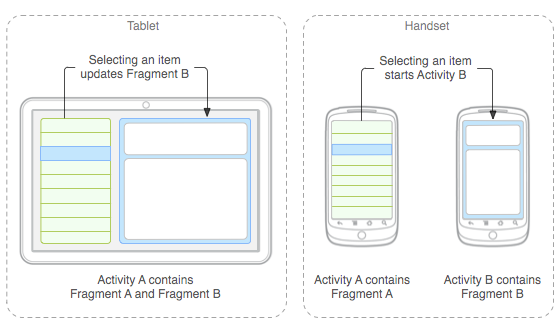
\includegraphics{fragments.png}
Перейдем к рассмотрению нашего ForecastFragment:
	\begin{lstlisting}
public class ForecastFragment extends Fragment implements LoaderManager.LoaderCallbacks<Cursor> {

    private static final int FORECAST_LOADER_ID = 0;

    private static final String[] FORECAST_COLUMNS = {
            WeatherContract.WeatherEntry._ID,
            WeatherContract.WeatherEntry.COLUMN_DATE,
            WeatherContract.WeatherEntry.COLUMN_DAY_TEMP,
            WeatherContract.WeatherEntry.COLUMN_NIGHT_TEMP,
            WeatherContract.WeatherEntry.COLUMN_WIND_SPEED,
            WeatherContract.WeatherEntry.COLUMN_DEGREES,
            WeatherContract.WeatherEntry.COLUMMN_WEATHER_ID
    };

    public static final int COLUMN_WEATHER_DATE = 1;
    public static final int COLUMN_WEATHER_DAY = 2;
    public static final int COLUMN_WEATHER_NIGHT = 3;
    public static final int COLUMN_WEATHER_WIND_SPEED = 4;
    public static final int COLUMN_WEATHER_WIND_DEGREES = 5;
    public static final int COLUMN_WEATHER_ID = 6;

    private ForecastAdapter mForecastAdapter;

    public ForecastFragment() { }

    @Override
    public void onActivityCreated(Bundle savedInstanceState) {
        super.onActivityCreated(savedInstanceState);
        getLoaderManager().initLoader(FORECAST_LOADER_ID, null, this);
    }

    @Override
    public View onCreateView(LayoutInflater inflater, ViewGroup container,
                             Bundle savedInstanceState) {
        super.onCreateView(inflater, container, savedInstanceState);

        View root = inflater.inflate(R.layout.fragment_main, container, false);
        ListView mListView = (ListView) root.findViewById(R.id.forecast_list_view);
        mForecastAdapter = new ForecastAdapter(getActivity(), null, 0);
        mListView.setAdapter(mForecastAdapter);
        return root;
    }

    ...
}
    \end{lstlisting}
Здесь мы переопределяем два метода класса Fragment - onActivityCreated и onCreateView. Первый вызывается после того, как завершен вызов метода onCreate у Activity, к которой прикреплен наш Fragment.\newline
onCreateView вызывается, когда фрагменту нужно нарисовать его UI в первый раз и возвращает View для UI фрагмента.\newline
Теперь добавим ForecastFragment на MainActivity:
	\begin{lstlisting}
public class MainActivity extends ActionBarActivity {

    private LocationManager mLocationManager;
    private PendingIntent mLocationChangedIntent;

    @Override
    protected void onCreate(Bundle savedInstanceState) {
        super.onCreate(savedInstanceState);
        setContentView(R.layout.activity_main);
        if (savedInstanceState == null) {
            getSupportFragmentManager().beginTransaction()
                    .add(R.id.container, new ForecastFragment())
                    .commit();
        }
        ...
    }
    ...
}
    \end{lstlisting}
Здесь мы получаем FragmentManager - интерфейс для взаимодействия с Fragment внутри Activity, и у него вызываем метод beginTransaction, который начинает конвейер операций с фрагментами, дальше добавляем новый ForecastFragment, указав контейнер, куда он отправится, и, наконец, исполняем все действия с помощью метода commit. По идентификатору R.id.container мы найдем layout для MainActivity, так что мы просто располагаем фрагмент на нем.

=======
    \begin{itemize}
	\item Весь UI в большинстве приложений распихан по фрагментам.
	\item Подробнее про Фрагменты можно почитать тут: \href{http://developer.alexanderklimov.ru/android/theory/fragments.php}{тык}
    \end{itemize}
>>>>>>> 7257234cd4f8a1229a5d50f3966045f111454229
\section{ListView \& Adapter}   
    Единственная компонента нашего фрагмента - это список, который отрисовывается с помощью ListView. \newline
    ListView и Adapter - это в некотором смысле андроидовская реализация того, что называют Model-View Controller.
    
    Идея в следующем - есть какая-то View, рисующая UI. Есть набор данных, по которым этот UI рисуется. И они разделены по разным классам. Таким образом, мы, например, можем подменить один View другим, не меняя модельку, в которой эти данные хранятся.

    \begin{itemize}
        \item Для того, чтобы рисовать списки, используют ListView.
        \item Adapter - класс, который предоставляет нам доступ к данным. А так как у нас есть база данных, то в нашем случае мы хотим, чтобы Adapter предоставлял нам доступ к нашей базе данных. Для этого в Android есть специальный класс, называемый CursorAdapter(он, например, при обновлении БД оповещает View об этом).
        \item При создании CursorAdapter необходимо переопределить несколько методов - public View newView(...), public void bindView(...).
        \item public View newView(Context context, Cursor cursor, ViewGroup parent) - создаёт новую View. Вызывается, когда для каких-то данных в ListView надо добавить новое View. context - для доступа к системным ресурсам. cursor - указывает на текущую строчку в базе данных(на ту строчку, для которой мы хотим создать новую View). parent - элемент, внутрь которого мы должны новую View положить.
        \begin{lstlisting}
@Override
public View newView(Context context, Cursor cursor, ViewGroup parent) {
    View view = LayoutInflater.from(context).inflate(R.layout.forecast_list_item_view,
            parent, false);
    view.setTag(new ViewHolder(view));
    return view;
}        
        \end{lstlisting}
        \item LayoutInflater - это сущность, которая по xml-описанию View создаёт эту View. 
        
        Пример xml-описания:
        \begin{lstlisting}
<?xml version="1.0" encoding="utf-8"?>
<LinearLayout
    xmlns:android="http://schemas.android.com/apk/res/android"
    android:orientation="horizontal"
    android:gravity="center_vertical"
    android:layout_width="match_parent"
    android:layout_height="wrap_content"
    android:layout_margin="20dp">

    <LinearLayout
        android:orientation="vertical"
        android:layout_width="0dp"
        android:layout_height="wrap_content"
        android:layout_weight="1">

        <TextView
            android:id="@+id/date"
            android:layout_width="wrap_content"
            android:layout_height="wrap_content"
            android:layout_margin="10dp"/>

        <TextView
            android:id="@+id/wind"
            android:layout_width="wrap_content"
            android:layout_height="wrap_content"
            android:layout_margin="10dp"/>

    </LinearLayout>

    <LinearLayout
        android:orientation="vertical"
        android:layout_width="0dp"
        android:layout_height="wrap_content"
        android:layout_weight="1"
        android:gravity="right">
        
        <ImageView
            android:id="@+id/icon"
            android:layout_width="wrap_content"
            android:layout_height="wrap_content"
            android:layout_margin="10dp"/>

        <TextView
            android:id="@+id/temp"
            android:layout_width="wrap_content"
            android:layout_height="wrap_content"
            android:layout_margin="10dp"/>

    </LinearLayout>

</LinearLayout>    
        \end{lstlisting} 
        
        Здесь, внешний LinearLayout - это такая Group, в которую добавленные элементы горизонтально(android:orientation="horizontal") ложаться друг за другом.
        
        Два внутренних LinearLayout - это аналогичные Group, только элементы ложаться по вертикали(android:orientation="vertical").
        
        TextView - это просто текст, ImageView - изображение.
        
        Надо заметить, что View - это какая-то рисуемая сущность, а Group - сущность разметки, то есть она размещает по каким-то правилам View или другие Group. Так вот все *Layout - это Group.
        
        У каждого элемента можно задать id, по которому впоследствии его можно будет найти(например, с помощью метода findViewById(int id) у Context. Без id элемент найти будет трудно, поэтому если какой-то элемент используется или изменяется в коде, ему обязательно нужно дать своё id.
        \item Можно размечать экран и с помощью кода, создавая Layout-ы и View на ходу, но xml в некотором смысле практичней, поскольку мы просто можем заменить один layout другим без изменения кода.
        \item Итак, LayoutInflater получает xml-файл, создаёт дерево объектов и возвращает корневой.
        \item Рядом с любой View мы можем хранить данные, добавляя их с помощью метода .setTag(Data data);
        \item ViewHolder, который мы добавляем в качестве дополнительной информации к View, один раз находит нужные нам View, которые мы будем изменять, и кеширует их, чтобы не приходилось какждый раз бегать по дереву объектов. Это действительно помогает, потому newView не всегда вызывается, когда на экране появляется очередная View. Андроид располагает небольшими ресурсами, поэтому созданные View он может переиспользовать, подав их же ещё раз на вход bindView. Например, так происходит при прокручивании списка.
        \item Следующий метод, про который нам надо поговорить - public void bindView(View view, Context context, Cursor cursor). bindView связывает View с данными, которые мы хотим на ней отобразить. То есть bindView в нашем случае должен заполнить поля у текстовых View, которые отвечают за температуру, чтобы они отображали актуальные данные:
 		\begin{lstlisting}
   @Override
    public void bindView(View view, Context context, Cursor cursor) {
        ViewHolder holder = (ViewHolder) view.getTag();

        long date = cursor.getLong(ForecastFragment.COLUMN_WEATHER_DATE);
        holder.date.setText(Utility.getFriendlyDayString(date));

        double day = cursor.getDouble(ForecastFragment.COLUMN_WEATHER_DAY);
        double nigh = cursor.getDouble(ForecastFragment.COLUMN_WEATHER_NIGHT);
        holder.temp.setText(Utility.getFormattedTemperature(day, nigh));

        double speed = cursor.getDouble(ForecastFragment.COLUMN_WEATHER_WIND_SPEED);
        double degrees = cursor.getDouble(ForecastFragment.COLUMN_WEATHER_WIND_DEGREES);
        holder.wind.setText(Utility.getFormattedWind(speed, degrees));

        int weatherId = cursor.getInt(ForecastFragment.COLUMN_WEATHER_ID);
        holder.icon.setImageResource(Utility.getWeatherConditionIcon(weatherId));
    }

    public static class ViewHolder {
        public TextView date;
        public TextView temp;
        public TextView wind;
        public ImageView icon;

        public ViewHolder(View view) {
            date = (TextView) view.findViewById(R.id.date);
            temp = (TextView) view.findViewById(R.id.temp);
            wind = (TextView) view.findViewById(R.id.wind);
            icon = (ImageView) view.findViewById(R.id.icon);
        }
    }        
        \end{lstlisting}
    \end{itemize}
    
    К CursorAdapter данные приходят от Cursor, он позволяет обращаться к различным методам Cursor: getDouble(), getPosition().
	
	Теперь посмотрим, что же происходит у нашего ForecastFragment в методе onCreateView:
	\begin{lstlisting}
@Override
public View onCreateView(LayoutInflater inflater, ViewGroup container,
                         Bundle savedInstanceState) {
    super.onCreateView(inflater, container, savedInstanceState);

    View root = inflater.inflate(R.layout.fragment_main, container, false);
    ListView mListView = (ListView) root.findViewById(R.id.forecast_list_view);
    mForecastAdapter = new ForecastAdapter(getActivity(), null, 0);
    mListView.setAdapter(mForecastAdapter);
    return root;
}    
    \end{lstlisting}
	Здесь мы:
\begin{itemize}
\item Вызываем метод родителя.
\item C помощью LayoutInflater получаем root нашей иерархии View.
\item С помощью root находим наш ListView.
\item Создаем ForecastAdapter и связываем его с View, для которой он отображает данные.
\item Возвращаем root.
\end{itemize}

    Для получения данных есть отдельный класс LoaderManager - это штука, которая управляет загрузками. Бывают встроенные Loader, если не устраивают, можно реализовать свой. Для этого нужно реализовать интерфейс LoaderCallbacks. Этот интерфейс вызывается, когда Loader загрузит какие-то данные.
	
    LoaderManager можно получить с помощью метода getLoaderManager() у Context. Так как возможна потребность в сразу нескольких загрузках, методу getLoader() у LoaderManager нужно передавать id, чтобы у нас была возможность отличать загрузки друг от друга.
    
    Для Cursor мы используем CursorLoader, чтобы загружать данные из нашего ContentProvider.
    
    А чтобы до нас доходили оповещения Loader о том, что что-то загрузилось, нужно реализовать методы у интерфейса LoaderCallbacks<Cursor>.
    
    Теперь посмотрим на полный код ForecastFragment:
    \begin{lstlisting}
public class ForecastFragment extends Fragment implements LoaderManager.LoaderCallbacks<Cursor> {

    private static final int FORECAST_LOADER_ID = 0;

    private static final String[] FORECAST_COLUMNS = {
            WeatherContract.WeatherEntry._ID,
            WeatherContract.WeatherEntry.COLUMN_DATE,
            WeatherContract.WeatherEntry.COLUMN_DAY_TEMP,
            WeatherContract.WeatherEntry.COLUMN_NIGHT_TEMP,
            WeatherContract.WeatherEntry.COLUMN_WIND_SPEED,
            WeatherContract.WeatherEntry.COLUMN_DEGREES,
            WeatherContract.WeatherEntry.COLUMMN_WEATHER_ID
    };

    public static final int COLUMN_WEATHER_DATE = 1;
    public static final int COLUMN_WEATHER_DAY = 2;
    public static final int COLUMN_WEATHER_NIGHT = 3;
    public static final int COLUMN_WEATHER_WIND_SPEED = 4;
    public static final int COLUMN_WEATHER_WIND_DEGREES = 5;
    public static final int COLUMN_WEATHER_ID = 6;

    private ForecastAdapter mForecastAdapter;

    public ForecastFragment() { }

    @Override
    public void onActivityCreated(Bundle savedInstanceState) {
        super.onActivityCreated(savedInstanceState);
        getLoaderManager().initLoader(FORECAST_LOADER_ID, null, this);
    }

    @Override
    public View onCreateView(LayoutInflater inflater, ViewGroup container,
                             Bundle savedInstanceState) {
        super.onCreateView(inflater, container, savedInstanceState);

        View root = inflater.inflate(R.layout.fragment_main, container, false);
        ListView mListView = (ListView) root.findViewById(R.id.forecast_list_view);
        mForecastAdapter = new ForecastAdapter(getActivity(), null, 0);
        mListView.setAdapter(mForecastAdapter);
        return root;
    }

    @Override
    public Loader<Cursor> onCreateLoader(int id, Bundle args) {
        String sortOrder = WeatherContract.WeatherEntry.COLUMN_DATE + " ASC";
        Uri weatherUri = WeatherContract.WeatherEntry.CONTENT_URI;

        return new CursorLoader(getActivity(), weatherUri, FORECAST_COLUMNS, null, null, sortOrder);
    }

    @Override
    public void onLoadFinished(Loader<Cursor> loader, Cursor data) {
        mForecastAdapter.swapCursor(data);
    }

    @Override
    public void onLoaderReset(Loader<Cursor> loader) {
        mForecastAdapter.swapCursor(null);
    }

}
    \end{lstlisting}
    Здесь мы:
\begin{itemize}
\item Инициализируем загрузчик и запускаем его в методе onActivityCreated c помощью метода initLoader у LoaderManager. Ему мы передаем три параметра - идентификатор загрузчика, дополнительные аргументы и LoaderCallbacks, которому LoaderManager сообщит о  изменении состояния загрузчика.
\item Описываем Loader, который мы хотим использовать для загрузки. Конструктору CursorLoader передается Context, ссылка на данные, указание на то, какие колонки вернуть, а также порядок их сортировки.

Внутри этого конструктора будет вызываться метод query() с теми же самыми параметрами у ContentProvider.
\item Обрабатываем две ситуации: onLoadFinished и onLoaderReset. В первой мы успешно загрузили информацию, тогда воспользуемся методом swapCursor у нашего адаптера, который освободит старые данные и будет работать с новыми.
\item Во втором варианте информация недоступна, и мы должны освободить старые данные с помощью mForecastAdapter.swapCursor(null).
\end{itemize}
 
\section{Директория res}
Она же ресурсы. Если мы хотим сохранить некоторую картинку, которой будет пользоваться наше приложение(например, иконку), или некоторый gif-файл, который мы хотим отображать на Activity, то их можно положить заранее сюда и доставать в тех местах в коде, где нам это нужно.Здесь хранятся:
\begin{itemize}
\item Иконки - в res/mipmap-hdpi, res/mipmap-mdpi, res/mipmap-xhdpi, res/mipmap-xxhdpi. Какая из них будет использована, зависит от размера экрана.
\item Изображения - в res/drawable. 
\item Layout - в res/layout.
\item Строки - в res/values/strings.xml.
\item Стили - в res/styles.
\item Содержимое меню приложения - в res/menu
\item Значения bool, color, dimen - в res/values.
\end{itemize}
Приведем пример того, как используются resources, а именно покажем, как их применять для локализации. \newline

Рассмотрим файл res/values/strings.xml некоторого приложения:
	\begin{lstlisting}
<resources>
    <string name="app_name">ActivityExample</string>

    <string name="hello_world">Hello world!</string>
    <string name="action_settings">Settings</string>
    <string name="title_activity_sms">SMSActivity</string>
</resources>
    \end{lstlisting}
Допустим, мы хотим получить строку, на которой написано "Привет, мир!" на английском, если в настройках телефона указан не французский язык, а если французский, то просто "Bonjour tout le monde!" и разместить на TextView:
	\begin{lstlisting}
TextView textView = findViewById(R.id.textView);
String helloWorld = getResources().getString(R.string.hello_world);
textView.setText(helloworld);
    \end{lstlisting}
Здесь мы:
\begin{itemize}
\item Находим с помощью метода findViewById(int id) у Context нашу TextView. 
\item Обращаемся к ресурсам с помощью метода getResources() у Context и находим там нашу строку с помощью метода getString(int id)
\item Размещаем строку на TextView.
\end{itemize}
Заметим, что здесь мы два раза пользуемся id - идентификатором, который есть как у View, так и у ресурсов. Получить идентификатор для строки, хранящейся в ресурсах, можно, написав R.string.*name*, где name соответствует полю name в xml-файле.\newline
Теперь хотим добавить вариант на французском. Для этого создадим директорию res/values-fr и в ней создадим файл strings.xml, внутри которого напишем:
	\begin{lstlisting}
<resources>
    <string name="app_name">ActivityExample</string>

    <string name="hello_world">Bonjour tout le monde!</string>
    <string name="action_settings">Settings</string>
    <string name="title_activity_sms">SMSActivity</string>
</resources>    
    \end{lstlisting}
Код оставим таким же, без изменений. Теперь, если на телефоне выставлен французский язык, на TextView будет размещена надпись по-французски, а если нет - то на английском. Аналогично можно создавать альтернативные ресурсы и для других языков.
\end{document}
